\documentclass[12pt, a4paper]{ctexart} % 直接使用中文文档类

% ---------- 页面设置 ----------
\usepackage{algorithm}      % 算法环境
\usepackage{algorithmic}    % 算法伪代码
\usepackage{amsmath, amssymb}   % 数学公式支持
\usepackage{geometry}
\usepackage{indentfirst}   % 让首段也缩进
\usepackage{graphicx}
\usepackage{amsfonts} % 或者使用 \usepackage{amssymb}////为了使用黑体字公式
\usepackage{booktabs}%三线表格式
\usepackage{float}  %固定图片

\setlength{\parindent}{2em} % 缩进2字符(1em≈1汉字宽度)
\geometry{left=3cm, right=2.5cm, top=2.5cm, bottom=2.5cm}

% ---------- 字体配置 ----------
\setmainfont{Times New Roman}          % 设置西文字体

% ---------- 段落格式 ----------
\linespread{1.5}                      % 1.5倍行距
\setlength{\parindent}{2em}           % 首行缩进

% ---------- 标题格式 ----------
\usepackage{titlesec}
\titleformat{\section}{\Large\bfseries\heiti}{\thesection}{1em}{}
\titleformat{\subsection}{\large\bfseries\heiti}{\thesubsection}{1em}{}

% ---------- 文档信息 ----------
\title{当可解释性遇到对抗性学习:
使用 SHAP 检测对抗性示例
签名}
\author{译者    Tinkle}
\date{\today}

\begin{document}
\maketitle{}
% ---------- 摘要页 ----------
\begin{abstract}
    最先进的深度神经网络(DNN)在解决许多复杂的实际问题时非常有效。然而,这些模型很容易受到对抗性扰动攻击,尽管在该领域开展了大量研究,但时至今日,在对抗性示例生成方法与检测和预防方法的猫鼠游戏中,对抗者仍占上风。在这项研究中,我们提出了一种新颖的检测方法,该方法使用为 DNN 分类器内部层计算的 Shapley Additive Explanations (SHAP) 值来区分正常输入和对抗输入。我们通过在流行的 CIFAR-10 和 MNIST 数据集上建立一个广泛的对抗性示例数据集来评估我们的方法,并训练一个基于神经网络的检测器来区分正常输入和对抗性输入。我们针对各种最先进的攻击所生成的对抗性示例评估了我们的检测器,结果表明它具有很高的检测准确率,并且对不同攻击方法生成的对抗性输入具有很强的泛化能力。索引词:对抗性学习、可解释人工智能、SHAP、深度学习。
\end{abstract}

% ---------- 正文部分 ----------
\section{介绍}
近年来,深度神经网络(DNN)学习算法被广泛用于解决各种复杂问题。其最大的影响体现在图像分类、物体识别、自然语言处理和恶意软件检测等领域。尽管 DNNs 性能出众,常常胜过人类专家,但它们很容易受到敌意扰动的影响。Szegedy 等人[1]首先发现,对抗性扰动是对 DNN 输入的轻微修改,会导致错误分类。例如,在图像分类领域,这种修改可能是像素颜色的微小调整,人类无法察觉,但却会导致最先进的分类器产生攻击者任意选择的输出。从那时起,有关对抗性示例的广泛研究主要集中在四个方向:对抗性示例生成方法[2]-[6]、提高 DNN 模型对对抗性示例的鲁棒性的防御措施[7]-[9]、对抗性示例检测[10]-[16]以及了解对抗性示例的性质和根本原因[6]、[17]-[19]。目前,攻击者在与防御者的军备竞赛中仍处于领先地位,最先进的防御系统在先进的自适应攻击面前显得力不从心[20]。因此,有效检测对抗性示例的能力仍是一个有待解决的问题。DNN 模型的另一个看似无关但却显著的缺点是难以解释其原理,甚至难以提供支持证据来证明其决策的合理性。这对其在生产级环境中的应用构成了重大障碍[21]。为此,人们正在可解释人工智能(XAI)领域投入大量研究力量,以提高人类解释 DNN 和其他机器学习模型所做决策的能力[22]-[25]。我们假设,模型的可解释性与对抗性实例之间存在着深刻的联系。直观地说,一个解释良好的模型应该对对抗性扰动具有相当的鲁棒性,因为对抗性输入会导致模型决策出现异常解释。我们在本文中的目标是揭示并利用这种联系,推动对抗性实例检测技术的发展。我们提出并评估了一种新颖的对抗性示例检测方法,该方法将 SHAP 可解释性技术 [25] 应用于 DNN 的倒数第二层,以创建 “XAI 签名”,并将其输入我们的检测器。我们使用 CIFAR10 [26] 和 MNIST [27] 数据集对我们提出的方法进行了评估,总体上遵循了 Carlini 等人 [28] 提出的严格的对抗性防御评估准则。评估结果表明,我们的方法在检测对抗性示例方面非常有效(AUC ̃97\%),并且在不同的对抗性示例生成算法中都有很好的泛化效果。出色的泛化结果支持了我们的假设,即我们的方法捕捉到了对抗性示例的内在属性。与先前的检测器相比,我们针对更广泛的对抗性攻击(白盒和黑盒)(包括已知的最强攻击)评估了我们的检测器,并在两种情况下都获得了非常高的检测 ROC-AUC 分数:由检测器经过训练的攻击方法生成的对抗性示例,以及由检测器未经过训练的攻击方法生成的对抗性示例。总而言之,我们在本研究中的主要贡献有两个方面:(1)我们引入了一种新型对抗示例检测方法,该方法具有令人印象深刻的检测性能,并证明了它在应对各种对抗性攻击时的高效性;(2)我们朝着揭示对抗学习与可解释人工智能之间的深层联系迈出了第一步。

\section{背景}
\subsection{对抗攻击 (Adversarial Attacks)}

对机器学习分类器的攻击,称为对抗性机器学习 (adversarial machine learning),通常发生在机器学习过程的两个主要阶段:\textbf{模型训练阶段}(又称数据投毒 (poisoning))。\textbf{分类阶段}(又称规避攻击 (evasion attack))。在本研究中,我们关注规避攻击,特别是检测对抗样本。规避攻击涉及**修改输入样本的特征,以欺骗模型的检测能力,这些修改后的样本被称为对抗样本 (adversarial examples)。

给定一个分类器 \( f: \mathbb{R}^n \to C \),其将输入样本 \( x \in \mathbb{R}^n \) 映射到可能的目标类别集合 \( C \) 中,并假设其正确的类别标签为 \( c \)。我们定义**对抗扰动 (adversarial perturbation)** \( \delta \in \mathbb{R}^n \),使得对抗样本 \( x' = x + \delta \) 满足:
\[
f(x') \neq c,
\]
\[
s.t. \quad ||\delta|| < \epsilon
\]
其中 \( ||\cdot|| \) 是一个距离度量,\( \epsilon > 0 \) 是允许的最大扰动大小。

尽管人眼难以察觉对抗扰动,但它足以使模型误分类。常见的对抗攻击使用的距离度量包括:
\begin{itemize}
    \item \( L_0 \) (改变的输入特征数量)。
    \item \( L_2 \) (标准欧几里得距离)。
    \item \( L_{\infty} \) (单个特征的最大变化)。
\end{itemize}

用于生成对抗样本的方法被称为对抗攻击 (adversarial attack)。其中:
\begin{itemize}
    \item 目标攻击 (targeted attack) 使得样本被误分类为特定类别。
    \item 非目标攻击 (non-targeted attack) 只需使样本被误分类为任何错误类别即可。
\end{itemize}

近年来,已经提出了许多生成对抗样本的方法,其中包括:
\begin{itemize}
    \item \textbf{快速梯度符号方法 (Fast Gradient Sign Method, FGSM)}:一种基本技术,通过沿着模型损失函数梯度方向执行单步扰动,其大小由最大允许扰动 \( \epsilon \) 控制。
    \item \textbf{基本迭代方法 (Basic Iterative Method, BIM) 及其变体投影梯度下降 (Projected Gradient Descent, PGD)} \cite{pgd}:一种自然扩展 FGSM 的方法,采用**多步 FGSM 更新**,其步长累积不超过最大允许扰动 \( \epsilon \)。
    \item \textbf{Carlini \& Wagner (C\&W) 攻击} \cite{cw}:通过优化问题构造对抗样本,并**使用精心设计的损失函数** 来最小化扰动。
\end{itemize}

对抗攻击可进一步分为:
\begin{itemize}
    \item 白盒攻击 (White-box Attack):攻击者可以完全访问分类模型,包括其内部结构、参数和权重。
    \item 黑盒攻击 (Black-box Attack):攻击者只能访问模型的输入和输出,无法查看其内部状态。
\end{itemize}

此外,对抗攻击的一个重要性质是可迁移性 (transferability),即:

- 针对一个模型生成的对抗样本可能**同样有效地欺骗其他模型。

- 这种特性允许攻击者在一个白盒模型上训练对抗样本,然后用于攻击其他黑盒模型。

\subsection{对抗防御 (Adversarial Defenses)}

目前已有的对抗防御方法可以分为:
\begin{itemize}
    \item 提高模型鲁棒性的方法,旨在使模型对对抗样本具有更强的抗性。
    \item 检测对抗样本的方法,通过分析输入数据的异常性或模型内部行为来识别对抗样本。
\end{itemize}

用于生成鲁棒模型的技术包括:
\begin{itemize}
    \item 对抗训练 (Adversarial Training) 。
    \item 防御性蒸馏 (Defensive Distillation) 。
    \item 梯度混淆 (Gradient Obfuscation) 。
    \item 特征压缩 (Feature Squeezing) 。
\end{itemize}

在本研究中,我们提出了一种检测对抗样本的方法。以往的大多数方法尝试识别输入数据中的异常性,或者分析模型内部行为(如隐藏层激活)。还有一些方法采取更主动的方式,如:
- 转换输入数据,使其更难以受到对抗攻击的影响。
- 修改训练过程,提高检测器的性能。

\subsection{理解对抗样本 (Understanding Adversarial Examples)}

Ilyas 等人 认为,对抗样本的存在实际上是数据集本身的固有特性,并引入了鲁棒特征 (robust features) 和非鲁棒特征 (non-robust features) 的概念:
- 非鲁棒特征:
  - 具有高度预测性,但对输入的微小扰动极其敏感,容易发生大幅度变化。
  - 例如,在图像分类任务中,一些特征可能在模型训练时具有较强的预测能力,但对人类而言是不可察觉的随机模式。
- 鲁棒特征:
  - 既具有高度预测性,又不容易因为输入的微小变化而发生改变。
  - 例如,识别汽车时,\textbf{“轮子”} 和 \textbf{“车窗”} 就属于鲁棒特征。

Ilyas 等人的研究表明:

- 对抗样本的存在,以及它们在不同分类模型间的可迁移性 (transferability),是由于数据集中存在非鲁棒特征。

- 由于非鲁棒特征在训练过程中具有极高的预测能力,因此模型高度依赖这些特征,使其易受对抗攻击影响。

- 即便微小的输入扰动,也可能导致模型高度依赖的非鲁棒特征发生剧烈变化,从而造成误分类。

\subsection{可解释性AI}
可解释人工智能(XAI)是机器学习领域的一个新兴研究领域,目的是让用户理解、信任并有效管理下一代人工智能解决方案。近年来开发的大多数 XAI 方法都是为了解释有监督的机器学习模型。例如,LIME方法介绍了使用局部模型解释预测;DeepLIFT方法通过网络中的所有神经元使用反向传播来解释输出;SHAP方法是一种统一的方法,旨在使用形状值解释模型输出--形状值是从博弈论中借用的概念,用于计算联盟中不同参与者的相对贡献。在 XAI 中,它们用于估算特定输入或神经元对模型决策的贡献。在基于深度学习模型的异常检测中,解释输出的必要性尤为重要,因为在这种情况下,通常并非所有异常类型都是已知的(已标记)。在这项研究中,我们使用了 SHAP DeepExplainer 方法,它是 SHAP 算法的一种变体,专门针对解释 DNN 模型进行了优化。

\section{相关工作}
以往的研究提出了检测对抗性示例的方法。这些工作的摘要见表 I。表中简明扼要地总结了每个检测器的检测概念、评估设置和结果。此外,我们还总结了每个检测器最重要的优缺点。在这项研究中,我们提出了一种新颖的检测对抗样本的方法,这是以前从未提出过的。此外,我们还进行了更全面的评估,检查了模型的交叉攻击泛化能力,并对更多不同类型的攻击进行了评估,从而为我们的模型适应现实世界挑战的能力提供了更大的信心。

\section{通过可解释性实现稳健性}
对抗性规避攻击会改变非稳健特征的值,而在很大程度上保留稳健特征。这是因为对稳健特征进行有效修改需要对输入进行重大更改。因此,我们假设,在对正常输入和对抗输入进行分类时,稳健特征与非稳健特征的重要性会有不同的模式,后者更依赖于非稳健特征。我们尝试利用可解释的人工智能方法(XAI)来解释模型预测,从而充分利用对抗性示例的这一假设属性。因此,对于每个要分类为对抗性或正常的输入,我们利用 SHAP  计算分类模型倒数第二层神经元的重要性得分。然后,我们将这些重要性分数作为对抗性示例检测器的特征。之所以要解释倒数第二层(而不是输入层),是因为这一层的神经元实际上构成了原始分类模型的高级特征。图 1 举例说明了我们的假设。在图的左侧,我们可以看到同一类别 “猫 ”的三个正常示例,而在右侧,我们可以看到另一类别 “汽车 ”的三个正常示例。在图的中间,我们可以看到 “汽车 ”类的一个正常(原始)示例,以及对该示例进行有针对性(目标类 “猫”)的 PGD L2 攻击后的扰动。在每幅图像(示例)下方,我们给出了图像的 SHAP XAI 签名,即签名中坐标(行 = $i$,列 = $j$)处的每个像素都包含神经元 $i$ 对目标类别 $j$ 的 SHAP 值。颜色的深浅表示正负贡献的大小,白色/透明像素表示没有任何贡献。从鸟瞰图中可以看出,同一类图像(汽车或猫)的 XAI 签名相似,而不同类别的图像则具有不同的 XAI 签名。还可以观察到,虽然原始和扰动的汽车示例看起来相同,但它们的 XAI 签名却不同。然而,仔细观察会发现更多耐人寻味的特性: 正常汽车的 XAI 签名中有五行相对独特(两行靠近顶部,两行靠近底部,一行靠近中间)。此外,这些行中的亮红色像素位于第 1 列和第 9 列,分别对应目标类别 “汽车 ”和 “卡车”。
\begin{figure}[h]
    \centering
    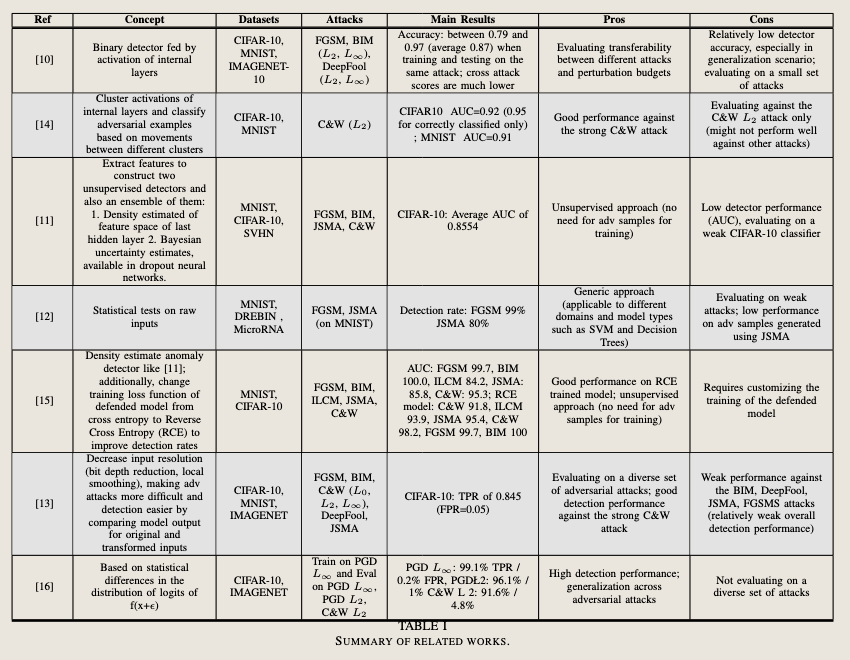
\includegraphics[width=0.9\textwidth]{img/adversaries_1.png}
\end{figure}
在图的左侧,三个正常猫的例子在 XAI 签名的中上部都有一坨外观相似的红色像素。转到对抗性汽车示例,我们可以看到它与正常汽车共享五行中的两行,与猫共享中上部的一坨红色像素。因此,“汽车 ”和 “猫 ”特征的混合在这个对抗示例的底层分类器决策中发挥了重要作用。虽然这只是一种推测,还需要进一步研究才能得出有力的结论,但我们假设这种行为完全符合稳健特征和非稳健特征的概念: 对抗性攻击未能改变的两行显著特征与 “汽车 ”类的稳健特征相对应,而其余三行消失的特征则与 “汽车 ”类的非稳健特征相对应。同样,从正常猫转移到对抗猫的红色肿块部分对应的是非稳健的 “猫 ”类特征,而没有转移的肿块部分对应的是稳健的 “猫 ”类特征。为了更深入地探索数据集,我们在训练集上训练了一个 UMAP [33] 降维器,并用它将测试集投影到训练集的嵌入空间上。在图 2 中,我们可以清楚地看到十个不同的正常样本集群(每个目标类别一个)和一个包含对抗样本的集群。根据这种分离,我们可以推断,计算出的 SHAP 值将成为我们检测器的良好特征。图 3 仅显示了投射到与图 2 相同的嵌入空间中的对抗样本。不同类型的对抗性示例在对抗性示例集群周围的广泛空间分散暗示我们,当我们的检测器在未经过训练的对抗性示例类型上进行测试时,它可以很好地泛化。


\section{建议的方法}
提出的解决方案包括三个主要阶段(图 4):创建正常和对抗示例的存储库、生成 XAI 签名和检测器构建。

\subsection{符号定义}
    \begin{itemize}
        \item \( f(\cdot) \) - 基于神经网络的分类器。
        \item \( f^{[i]}(\cdot) \) - 第 \( i \) 层神经网络的输出(\( 0 \leq i \leq l \)),其中 \( f^{[0]}(\cdot) \) 是输入层,\( f^{[l]}(\cdot) \) 是最终的 softmax 输出。
        \item \( x \) - 输入向量。
        \item \( Y(x) \) - 输入样本 \( x \) 的真实类别标签。
    \end{itemize}

\subsection{构建正常样本和对抗样本存储库}
在本阶段,我们生成一个存储库,包括正常样本和对抗样本:
    \begin{itemize}
        \item 正常样本从数据集中随机采样,并用于训练分类器 \( f(\cdot) \)。
        \item 对抗样本通过多种最先进的对抗攻击算法生成。 
    \end{itemize}

当生成对抗样本时,必须调整攻击的超参数,如:
\begin{itemize}
    \item 距离度量(如 \( L_0, L_1, L_2, L_{\infty} \))。
    \item 扰动预算(perturbation budget)。
    \item 迭代次数(number of iterations)。
    \item 攻击步长(attack step size)。
\end{itemize}

调整不同超参数会导致不同的攻击方式,从而提高检测模型的泛化能力。

算法 1 详细描述了生成对抗样本的过程。每次迭代中,算法:
\begin{enumerate}
    \item 随机选择一个正常样本。
    \item 选择一个攻击方法、距离度量和攻击偏好参数。
    \item 选择一个不同于真实标签的目标类别。
    \item 执行攻击,生成对抗样本。
    \item 如果生成的样本成功误导分类器,即分类结果与目标类别匹配,则存储该对抗样本。
\end{enumerate}

\begin{figure}[h]
    \centering
    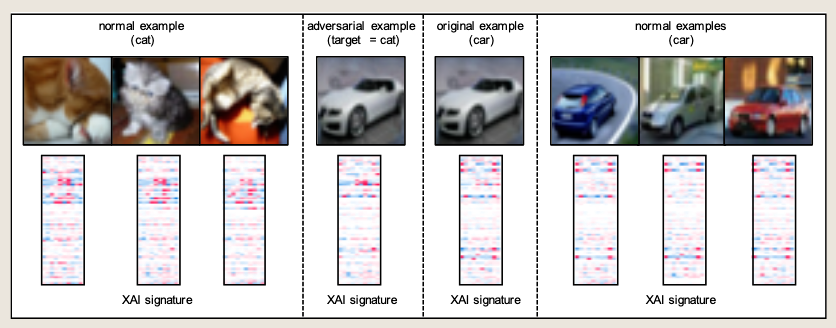
\includegraphics[width=0.9\textwidth]{img/adversaries_2.png}
    \caption{说明来自不同类的示例以及原始示例和对抗示例的 XAI 签名。}
\end{figure}

\begin{figure}[h]
    \centering
    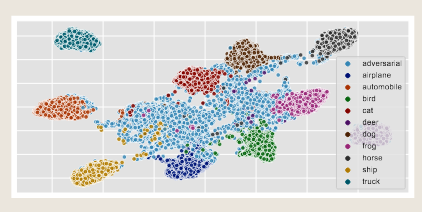
\includegraphics[width=0.9\textwidth]{img/adversaries_3.png}
    \caption{正常和对抗样本的 XAI 特征的 UMAP 可视化 (CIFAR-10)}
\end{figure}

\begin{figure}[h]
    \centering
    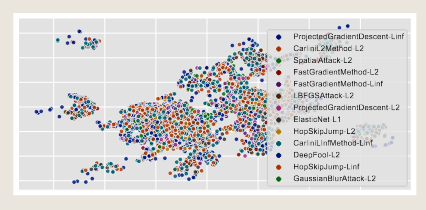
\includegraphics[width=0.9\textwidth]{img/adversaries_4.png}
    \caption{不同对抗样本的 XAI 特征的 UMAP 可视化 (CIFAR-10)}
\end{figure}


\subsection{生成 XAI 特征标识}
在本阶段,我们使用 SHAP 方法为数据集中的每个样本(包括正常样本和对抗样本)生成 XAI 特征标识。具体而言,我们应用 SHAP DeepExplainer 计算 SHAP 值,以解释神经网络的倒数第二层 \( f^{[l-1]}(\cdot) \) 的神经元。
\begin{algorithm}
    \caption{生成对抗样本}
    \begin{algorithmic}[1]  % 启用行号
    \STATE \textbf{Input:} $X_{normal}, L, M, D, P(m), f(\cdot), i$
    \STATE $X_{adversarial} \gets \emptyset$
    \WHILE{$i > 0$}
        \STATE $x \gets$ RandomSample($X_{normal}$)
        \STATE $m \gets$ RandomSample($M$)
        \STATE $d \gets$ RandomSample($D$)
        \STATE $p \gets$ RandomSample($P(m)$)
        \STATE $target \gets$ RandomSample($L \setminus Y(x)$)
        \STATE $x^* \gets m(x, d, p, target, f(\cdot))$
        \IF{$f(x^*) == target$}
            \STATE $X_{adversarial} \gets X_{adversarial} \cup x^*$
        \ENDIF
        \STATE $i \gets i - 1$
    \ENDWHILE
    \STATE \textbf{Return} $X_{adversarial}$
    \end{algorithmic}
\end{algorithm}
\begin{figure}
    \centering
    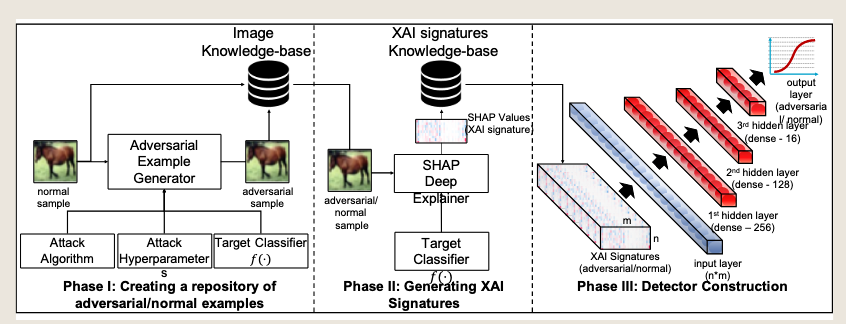
\includegraphics[width=0.9\textwidth]{img/adversaries_5.png}
    \caption{检测器训练过程。}
\end{figure}

对于每个输出类别,SHAP 计算 \( n \) 个 SHAP 值,其中 \( n \) 代表目标类别的数量。最终,每个样本的 XAI 特征标识由所有 SHAP 值拼接为一个向量,即:
\[
\text{signature} = n * |f^{[l-1]}(\cdot)|
\]
\subsection{训练检测器}
在本阶段,我们训练一个**二分类检测器**,用于区分正常样本和对抗样本:
\begin{itemize}
    \item 训练过程中,使用生成的数据集中的 SHAP 值作为特征。
    \item 训练一个标准的监督学习分类器,以检测对抗样本。
\end{itemize}

在推理阶段(inference phase):
\begin{enumerate}
    \item 计算输入样本的 SHAP 值,生成 XAI 特征标识。
    \item 将 XAI 特征标识输入检测器。
    \item 依据检测器输出,判断该样本是正常样本还是对抗样本。
\end{enumerate}

\section{评估}
在评估中,我们旨在回答以下两个研究问题: 

问题1:当训练集和测试集包含使用相同攻击和参数生成的对抗示例时,检测器的基准性能如何?

问题2:检测器能否泛化到由训练期间未知的攻击生成的对抗示例?
\subsection{评估设置}
我们使用以下两个图像分类使用案例对我们提出的检测方法进行了评估: [CIFAR,ResNet56]CIFAR-10数据集[26]与ResNet-56分类模型[34]。该模型在 CIFAR-10 测试集上达到了 93.39\% 的准确率。[MNIST,CNN]MNIST手写数字数据集[27],模型架构来自 Keras MNIST 示例 (https://keras.io/examples/mnist cnn/)。该模型在 MNIST 测试集上的准确率达到 99.25\%。 对抗示例生成 我们使用 Foolbox [35] 和 Adversarial Robustness Toolbox [36] 框架生成对抗示例。SHAP 解释是使用 SHAP 框架[25]生成的。表 2 列出了用于训练和测试检测模型的正常样本和对抗样本的数量(针对 CIFAR-10 和 MNIST 数据集)。
\begin{figure}[H]
    \centering
    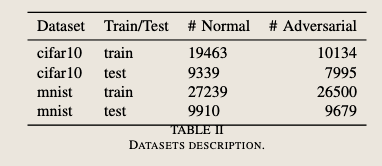
\includegraphics[width=0.9\textwidth]{img/adversaries_6.png}
    \caption{数据集描述}
\end{figure}
我们使用了多种攻击方法(见图 6)来生成对抗示例。 SHAP 值计算 对于 [CIFAR,ResNet]模型,我们在该模型的最后一层(也是唯一一层)全连接层上计算 SHAP 值,该层有 64 个神经元。这样,每个样本共有 640 个特征(10 个目标类别中的每个类别有 64 个特征)。对于 [MNIST,CNN]模型,我们在模型的最后一个全连接层上计算 SHAP 值,该层有 128 个神经元,每个样本共有 1280 个特征。

训练对抗示例检测器 在每次实验中,我们都会从生成的存储库中获取相关的 SHAP 值,从而生成特定于实验的训练集和测试集。使用 SHAP 值作为特征,我们训练了一个具有三个隐藏层(分别有 256、128 和 16 个神经元)的全连接前馈神经网络,所有隐藏层都具有 ReLU 激活单元和 Sigmoid 输出。我们使用 80/20 随机分割法将训练集分成训练子集和验证子集,并使用默认参数的 AdaBound 优化器[37]。我们最多训练 500 个历时,并设定了提前停止条件,即监控二元交叉熵验证损失,如果在过去 20 个历时内没有改善,则决定停止训练。

\subsection{结果与讨论}
问题 1:检测器的基线性能: 对于每个数据集和模型对(即 [CIFAR,ResNet56]和 [MNIST,CNN]),我们构建了训练集和测试集,具体如下。对于训练集,我们使用了所选数据集(CIFAR-10 或 MNIST)的所有正常和对抗训练样本。同样,对于测试集,我们使用了所选数据集的所有正常和对抗测试样本。训练集/测试集中的每个样本都使用其 SHAP 值来表示,对于对抗样本,类标签设置为 “1”,否则为 “0”。在图 5 中,我们展示了 ROC 和精确率曲线,以及这些曲线下的面积(AUC-ROC 和 AUC-PR)。可以看出,在 CIFAR-10 和 MNIST 数据集上,所提出的方法具有很高的检测性能,AUC-ROC 分别为 0.966/0.967,AUC-PR 分别为 0.958/0.961。
\begin{figure}[H]
    \centering
    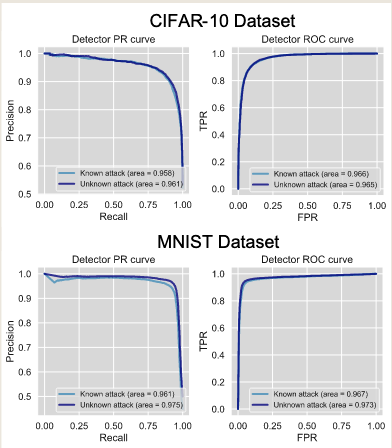
\includegraphics[width=0.8\textwidth]{img/adversaries_7.png}
    \caption{在 CIFAR-10 和 MNIST 数据集上评估了所提出的检测器的 ROC 和 PR 曲线。}
\end{figure}
我们还探讨了不同攻击方法的具体检测率。在图 6 中,我们展示了每种攻击方法的检测器的 TPR。结果显示,即使 FPR 为 0.05,大多数攻击的 TPR 也很高。
\begin{figure}[H]
    \centering
    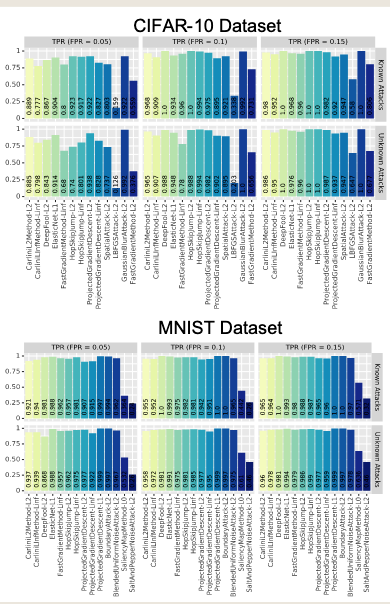
\includegraphics[width=0.8\textwidth]{img/adversaries_8.png}
    \caption{数据集描述}
\end{figure}


问题 2:不同攻击类型的通用性: 该评估模拟了这样一种场景:在已知攻击的对抗性示例基础上训练的检测器遇到了由未知攻击生成的对抗性示例。给定目标数据集和模型后,我们将其训练集和测试集按照(算法、度量)对进行划分,从而得到一个训练/测试子集集合。我们对每个测试子集进行随机欠采样,以平衡其中正常示例和对抗示例的数量。然后,我们采用 “排除法”,即对于每个(算法、度量标准)配对,我们在除该配对之外的所有训练样本上训练检测器,并仅在该配对生成的对抗性示例上进行评估。与前一个研究问题类似,我们评估了检测器的总体性能(图 5),以及每种攻击方法的单独性能(图 5)。可以看出,检测未知攻击的总体性能与已知攻击非常相似(CIFAR-10 和 MNIST 数据集的 AUC-ROC 分别为 0.965/0.973 和 AUC-PR 分别为 0.961/0.975)。同样,即使在 FPR 为 0.05 的情况下,所提出的方法在大多数攻击中也表现出很高的性能。
\section{结论和未来工作}
我们的实验结果验证了我们的方法有能力检测由各种最新攻击产生的对抗性示例(问题 1)。我们的实验结果表明,当检测器遇到未经过训练的攻击所产生的对抗性示例时,检测器也能很好地进行泛化(问题 2)。这些结果支持了我们的假设,即分类模型倒数第二层的 SHAP 值模式、鲁棒性与非鲁棒性特征对分类结果的重要性分布以及检测对抗性示例的能力之间存在联系。虽然我们的检测方法是基于监督学习模型的,需要利用各种攻击生成大量的对抗示例训练集,但良好的泛化结果意味着可以设计一种基于相同特征的半监督检测方法,以简化检测器的训练过程并进一步提高其性能。我们提出的方法可以进一步扩展为一个通用框架,让人联想到防病毒或 IDS 系统,这些系统会持续收集和分析良性和恶意样本,提取签名,并根据这些签名将样本分类为恶意或良性,或转发给人工分析。这样的框架既采用了本文讨论的基于 SHAP 的签名,也采用了其他最先进的检测器中使用的签名,可以提高防御对抗性示例的实际能力。在本文中,我们为理解模型解释与特征鲁棒性之间的联系迈出了第一步。对这种联系进行严格研究,既有利于提高我们探测器的性能,也有利于更好地理解对抗性示例的本质。未来的其他工作可能包括 (1) 在更多数据集(来自其他领域)和分类模型上测试我们的方法;(2) 评估检测器在底层分类模型之间的可转移性;(3) 评估我们的方法是否能抵御根据我们的检测器进行调整的定制攻击(这并非易事,因为 SHAP 值的计算不可微)。

\end{document}
